% arara: xelatex: { shell: yes }
% arara: makeglossaries
% arara: biber
% arara: xelatex: { shell: yes }
% arara: xelatex: { shell: yes }

\documentclass[thesis=M,english,hidelinks]{template/FITthesisXE}

\usepackage{graphicx}	% graphics files inclusion
\usepackage{dirtree}	% directory tree visualisation
\usepackage{longtable}	% tables which Pandoc use
\usepackage{lscape}		% to be able to rotate stuff
\usepackage{metalogo}	% for \XeLaTeX
\usepackage{xcolor}
\usepackage{blindtext}

\newcommand{\todo}[1][TODO]{\textcolor{red}{\textbf{[[#1]]}}}
\newcommand{\blind}[1][1]{\textcolor{gray}{\Blindtext[#1][1]}}
\setlength{\fboxsep}{0.005pt}
\newcommand{\tmpframe}[1]{\fbox{#1}}
%\renewcommand{\tmpframe}[1]{#1}  % uncomment to disable borders around images
\newcommand{\todoimg}[1][1]{%
  \begin{figure}[htbp]
    \centering
    \tmpframe{
\includegraphics[width=#1\linewidth]{images/placeholder-image}}
    \caption{\label{fig:TODO} \todo[write title]}
  \end{figure}
}

\newminted{r}{frame=single,framerule=0pt,framesep=3pt,bgcolor=codebg}
\newmintinline{r}{bgcolor=codebg}  % no frame? :(

\bibliography{library.bib}

\makeglossaries
\newacronym{API}{API}{Application programming interface}
\newacronym{CLI}{CLI}{Command Line Interface}
\newacronym{CRAN}{CRAN}{The Comprehensive R Archive Network}
\newacronym{GNU}{GNU}{GNU's Not Unix!}

\glsaddall	% add even unused acronyms

% % % % % % % % % % % % % % % % % % % % % % % % % % % % % % 

\acknowledgements{\todo[acknowledgements]
\blind[1]
}
\abstractEN{R is a dynamic programming language that, despite being over 20 years old, is still widely used. RIR is an alternative to its bytecode compiler and interpreter that aims to facilitate adding static analyses and optimization passes easily. RIR is under development and does not currently match the performance of standard R. This thesis attempts to amend the situation. It extends the RIR internal representation, adds new features to its compiler and refactors its interpreter. The average slowdown versus standard R is brought down by about one half in the Shootout benchmarks.
}
\abstractCS{R je dynamicý programovací jazyk, navzdory svému stáří dnes stále oblíbený. RIR je alternativní implementace kompilátoru a interpretu R bajtkódu, která umožňuje snadno provádět statickou analýzu a přidávat optimalizace. RIR je ve vývoji a zatím nedosahuje výkonu standardního R. Tato diplomová práce se pokouší přiblížit výkon RIR k~výkonu standardního R. V~jejím rámci byly přidány nové instrukce do RIR bajtkódu a nová funkcionalita do jeho kompilátoru a došlo k~přepracování jeho interpretu. Průměrné zpomalení na sadě benchmarků Shootout proti standardnímu R bylo sníženo o~polovinu.
}
\title{Improvements of the RIR bytecode toolchain}
\authorGN{Jan}
\authorFN{Ječmen}
\authorWithDegrees{Bc. Jan Ječmen}
\author{Jan Ječmen}
\supervisor{Ing. Petr Máj}
\keywordsEN{R language, RIR, bytecode compiler \& interpreter, optimizations}
\keywordsCS{jazyk R, RIR, kompilátor \& interpret bajtkódu, optimalizace}
\department{Department of Theoretical Computer\newline Science}
\placeForDeclarationOfAuthenticity{Prague}
\declarationOfAuthenticityOption{1}
\website{https://github.com/JanJecmen/dip}
\assignment{assignment.pdf}


\begin{document}

\hyphenation{frame-work}


\begin{introduction}
\label{introduction}
\todo[write intro]

\todo[cite: https://www.tiobe.com/tiobe-index/
http://pypl.github.io/PYPL.html]

\blind[3]
\todo[write about structure]
\blind[1]

\end{introduction}

\chapter{About GNU R\label{gnur}}

GNU~R \autocite{about} is a programming language used mainly for statistical computations.\footnote{Homepage: \url{https://www.r-project.org/}} It is an open-source dialect of S, an older statistical language created in 1976 by John Chambers at Bell Laboratories. R~has been around from 1993 and was designed by Ross Ihaka and Robert Gentleman, both recognized statisticians. It is a part of the GNU software family and is still actively developed by the R~Core Team today. It is a popular alternative to the other major implementation of the S~language, S-PLUS, which is a commercial version shipped by TIBCO Software Inc.

R comes with a software environment built around it, which allows for easily manipulating data, carrying out computations and producing quality graphical outputs such as plots and figures. Although at its heart R is used via a command line interface, there are also more user-friendly graphical IDEs available. One of the most widely used is RStudio that provides, for example, syntax highlighting and quick access to documentation through a web-like browser.\footnote{Homepage: \url{https://www.rstudio.com/}} This, together with R's readable syntax and a vast collection of extension packages available through The Comprehensive R~Archive Network (CRAN) makes it possible for new users to step in and start working quickly.

% % % % % % % % % % % % % % % % % % % % % % % % % % % % % % 

\section{Language features of R}

This section was written while consulting \autocite{hadley, design, inferno, rint, rlang}.

R is, as far as programming languages go, very interesting and has some quite unusual semantic features. It is an interpreted language, and is dynamically typed and garbage collected. It supports multiple programming paradigms: users can use procedural imperative style, but at the same time R provides an object system for object oriented programming, and is heavily influenced by functional programming languages, notably Scheme (a~dialect of Lisp).\footnote{In fact, R has multiple OO systems: 3 builtin and others available as packages, such as R.oo (\url{https://cran.r-project.org/web/packages/R.oo/}) or R6 (\url{https://cran.r-project.org/web/packages/R6/}).}

Functions are, in accordance with functional languages, first-class values, so they can be passed around as call arguments, returned as results of function calls and created dynamically at runtime. R uses lexical scoping (which it adopted from Scheme) and R functions are closures that capture their enclosing environment at creation time. Arguments are passed by value (although a variant of reference counting is implemented, so that deep copies are only created as needed, e.g., when an object is modified).

Functions are by design anonymous, i.e., they are not named when created. This is unlike many languages (e.g., C or Python) and follows the approach of lambda calculus. Instead of creating named functions, R programmers create anonymous ones and, if they choose so, then use regular assignment to bind them to names. Example can be seen in listing \ref{lst:anon-func}.

\begin{listing}[htbp]
  \caption{\label{lst:anon-func}Anonymous function}
  \begin{rcode}
> (function(x) x + 1)(2)
[1] 3
> f <- function(x) x + 1
> f(2)
[1] 3
  \end{rcode}
\end{listing}

Interestingly, everything that happens in R is in fact a function call. This goes as far as all control flow statements and arithmetic operators being just syntactic sugar for function calls, as can be seen in listing \ref{lst:funcall}.\footnote{As a side note, backticks are used in R to denote symbols (i.e. names). Because some symbols have special syntactic meaning (like the \rinline/`+`/ being an infix binary operator), they can cause a syntax error if they appear unquoted in a place where the parser does not expect them.} In this spirit, even assigning into a variable, evaluating a block of code inside curly brackets or grouping expressions with parentheses translate to calling the respective functions. As such, everything can be redefined, as in listing \ref{lst:paren-redef}.

\begin{listing}[htbp]
  \caption{\label{lst:funcall}All that happens in R is function call}
  \begin{rcode}
> is.function(`while`)
[1] TRUE
> is.function(`break`)
[1] TRUE
> is.function(`if`)
[1] TRUE
> `if`(TRUE, 1, 0)
[1] 1
> `if`(FALSE, 1, 0)
[1] 0
> `+`
function (e1, e2)  .Primitive("+")
> `+`(1, 2)
[1] 3
  \end{rcode}
\end{listing}

\begin{listing}[htbp]
  \caption{\label{lst:paren-redef}Redefinition of parentheses grouping}
  \begin{rcode}
> ((0))
[1] 0
> `(` <- function(x) x + 1
> ((0))
[1] 2
  \end{rcode}
\end{listing}

All actual arguments to a function are lazy evaluated by default. When applying a closure, parameters are wrapped in promises. A~promise is an object that contains the unevaluated expression and an environment in which the expression should be evaluated. Promises are only evaluated when the value is actually needed (which is called forcing the promise). Also, once the promise is forced, it remembers the result, so that subsequent uses of the value do not evaluate the expression again.

Delayed evaluation is demonstrated in listing \ref{lst:prom-lazy}, where the function in question only evaluates its first argument and does not touch the second. For the first call, the block of code in the curly brackets is never executed and so the side-effect of printing a greeting does not happen.\footnote{\rinline/cat/ is short for \emph{concatenate and print}.} In the second call, the arguments are swapped, and the side-effect can be observed in the output. It is possible to pass a~block of code as a~function argument, since the \rinline/`{`/ is bound to a function that sequentially evaluates all its arguments and returns as its result the value of the last expression (or \rinline/NULL/ if no expressions are passed in).

\begin{listing}[htbp]
  \caption{\label{lst:prom-lazy}Promise lazy evaluation}
  \begin{rcode}
> f <- function(a, b) a
> f(1, {cat("Hello\n"); 2})
[1] 1
> f({cat("Hello\n"); 2}, 1)
Hello
[1] 2
  \end{rcode}
\end{listing}

R supports assignment which enables programmers to change a function's local state by modifying its bindings and thus the imperative programming style.\footnote{An interesting quirk is R's left to right assignment: the code \rinline/1 -> x/ assigns to \rinline/x/ and is equivalent to \rinline/x <- 1/.} Also, the superassignment operator \rinline/`<<-`/ brings into play non-local side-effects (as shown in listing \ref{lst:superassign}).

\begin{listing}[htbp]
  \caption{\label{lst:superassign}Superassignment}
  \begin{rcode}
> x <- 1
> f <- function() {
+     x <- 2  # local
+     x <<- 3  # lookup in the enclosing environment
+     x  # local
+ }
> x
[1] 1
> f()
[1] 2
> x
[1] 3
  \end{rcode}
\end{listing}

The basic data type in R is an atomic vector. Vectors are collections of homogeneous values (a given vector can only hold objects of one particular type), that preserve the order of their elements. R also provides a list type which is heterogeneous. Higher-dimensional types such as matrices and data frames, as well as objects, are internally built on vectors and lists. Vectors can be created in R by calling the function \rinline/c/.\footnote{The name stands for \emph{combine}.}

Atomic vectors can have one of these six types: logical, integer, double, character, complex and raw. Since R targets data analysis, a special ``not~available'' value \rinline/NA/ is provided for these. Because all values in a vector must be of the same type, R performs coercion when an attempt is made to combine vectors of different types. In listing \ref{lst:coercion}, combining a numeric vector with a character vector results in a character vector, and summing a logical vector coerces to integers (\rinline/TRUE/ becoming \rinline/1/ and \rinline/FALSE/ becoming \rinline/0/).

In R there are no scalar types, as scalar values, such as individual numbers and strings, are considered to be vectors of length one. This holds for character vectors, too, which can cause confusion if one expects C-like behavior of strings and tries subscripting, because in R the subscript belongs to the vector that holds the string and not the string itself.\footnote{In such a case, one needs to use the \rinline/substr/ function.}

\begin{listing}[htbp]
  \caption{\label{lst:coercion}Coercion to the most flexible type}
  \begin{rcode}
> x <- c(1, 2, 3)
> y <- c("a", "b", "c")
> typeof(x)
[1] "double"
> typeof(y)
[1] "character"
> c(x, y)
[1] "1" "2" "3" "a" "b" "c"
> typeof(c(x, y))
[1] "character"
>
> sum(c(TRUE, TRUE, FALSE, TRUE))
[1] 3
  \end{rcode}
\end{listing}

Despite its inspiration in functional world, R does not optimize tail recursion, which is the standard approach in functional languages since they typically use recursion in the place of iterative loops. Instead, R encourages vectorized operations. Hence, most of R builtin functionality works element-wise with vectors, while recycling the elements as needed (e.g., when adding vectors of different lengths). This is demonstrated in listing \ref{lst:recycling}, where R even issues a warning about recycling.

\begin{listing}[htbp]
  \caption{\label{lst:recycling}Recycling shorter vector}
  \begin{rcode}
> numeric(10)
 [1] 0 0 0 0 0 0 0 0 0 0
> 1:3
[1] 1 2 3
> numeric(10) + 1:3
 [1] 1 2 3 1 2 3 1 2 3 1
Warning message:
In numeric(10) + 1:3 :
  longer object length is not a multiple of shorter object length
  \end{rcode}
\end{listing}

In R, every object can have arbitrary attributes associated with its data. Attributes are basically a hidden map that assigns names to values. Some of the most important attributes are names (a character vector that assigns names to elements), dimensions (a vector specifying the dimensions and thus effectively distinguishing vectors from matrices and arrays) and class (for implementing one of R's object systems). Attributes are used a lot in R for many purposes and extensions as they provide a way of encoding arbitrary additional metadata for objects. As an example, in listing \ref{lst:attributes} a vector of 4 elements is created, then changed into a two by two matrix and finally changed back to vector (that also has its elements named).\footnote{Here it can be seen here that R uses column-major order for storing the elements.}

\begin{listing}[htbp]
  \caption{\label{lst:attributes}Object attributes}
  \begin{rcode}
> x <- 1:4
> x
[1] 1 2 3 4
> attr(x, "dim") <- c(2, 2)
> x
     [,1] [,2]
[1,]    1    3
[2,]    2    4
> attr(x, "dim") <- c(4)
> attr(x, "names") <- c("a", "b", "c", "d")
> x
a b c d 
1 2 3 4 
  \end{rcode}
\end{listing}

True to its dynamic nature, R is very liberal in handling arguments in function calls. The language supports both positional and named matching of arguments, as well as default argument values. R even understands when the argument names are abbreviated, as long as the arguments can still be uniquely matched.

Moreover, R lets users call functions and not provide the specified arguments. It is only while executing the function body that the missing arguments may (or may not) cause an error. Variable number of arguments is supported as well by using the ellipsis \rinline/`...`/. The ellipsis in an argument list matches any number of arguments, and later in the function body refers to the list of matched arguments. Special symbols can be used to access the ellipsis arguments, such as \rinline/`..1`/, \rinline/`..2`/, etc. Argument handling is demonstrated in listing \ref{lst:args}.

\begin{listing}[htbp]
  \caption{\label{lst:args}Argument handling}
  \begin{rcode}
> f <- function(a, b, a.very.long.argument.name)
+     a.very.long.argument.name
> f(1, 2, 3)
[1] 3
> f(a = 3)
Error in f(a = 3) : 
  argument "a.very.long.argument.name" is missing, with no default
> f(a. = 3)
[1] 3
>
> f <- function(a, b) a
> # b is not required
> f(1)
[1] 1
> # a is required
> f()
Error in f() : argument "a" is missing, with no default
> f(b = 2)
Error in f(b = 2) : argument "a" is missing, with no default
>
> f <- function(...) ..2
> f()
Error in f() : the ... list does not contain 2 elements
> f(1, 2, 3, 4, 5)
[1] 2
  \end{rcode}
\end{listing}

As was already mentioned, R has multiple object systems. The simplest is called S3 and it uses a class attribute to implement ad hoc polymorphism (also known as function or operator overloading). It does not have formal classes, but instead uses a special function called a~generic function that decides what to call based on the value of the class attribute. A~typical example is printing, where the \rinline/print/ function is generic and its body consists of a call to a dispatcher \rinline/UseMethod("print")/. Specialized versions for different types can be defined, such as \rinline/print.data.frame/ for data frames, or, given an object with class set to \rinline/"foo"/, \rinline/print.foo/ (as is shown in listing \ref{lst:s3}).

\begin{listing}[htbp]
  \caption{\label{lst:s3}S3 object system}
  \begin{rcode}
> x <- list()
> class(x) <- "foo"
> print(x)
list()
attr(,"class")
[1] "foo"
> print.foo <- function(...) cat("Printing foo!\n")
> print(x)
Printing foo!
  \end{rcode}
\end{listing}

S4 is a more formal system than S3, and it allows for true class definitions, describing class representation and inheritance. It has multiple dispatch, which means that dispatchers can pick which method to call based on multiple arguments. R also has reference classes that implement message passing style. Their objects are modified in place (as opposed to the standard pass by value semantics).

An important and powerful feature of R is its subsetting and subset assignment mechanics. Parts of objects can be retrieved and even changed by the operators \rinline/`[`/, \rinline/`[[`/ and \rinline/`$`/. These behave differently for different types of objects.

The first version is a general subset function that supports all kinds of indexing.\footnote{As opposed to many languages (e.g., C or Python), R starts indexing elements from 1 instead of 0.} For example, integer vector specifies which elements to get and in what order, even allowing duplication. If negative indices are used, these elements are omitted from the result. Logical vectors can be used to select only elements at positions where \rinline/TRUE/ occurs. If the object is named, character vectors can be used to select by name. In combination with assignment (and superassignment), objects can be modified. Subsetting works also for higher-dimensional structures by simply providing indices for each dimension, separated by commas. Some examples are in listing \ref{lst:subset1}.

\begin{listing}[htbp]
  \caption{\label{lst:subset1}Basic subsetting / subassignment}
  \begin{rcode}
> x <- 101:110
> x
 [1] 101 102 103 104 105 106 107 108 109 110
> x[c(3, 5, 1, 1)]
[1] 103 105 101 101
> x[-c(2, 3, 8)]
[1] 101 104 105 106 107 109 110
> x > 105
 [1] FALSE FALSE FALSE FALSE FALSE  TRUE  TRUE  TRUE  TRUE  TRUE
> x[x > 105]
[1] 106 107 108 109 110
> x[x %% 2 == 0] <- NA
> x
 [1] 101  NA 103  NA 105  NA 107  NA 109  NA
> m <- matrix(1:9, ncol = 3)
> m
     [,1] [,2] [,3]
[1,]    1    4    7
[2,]    2    5    8
[3,]    3    6    9
> m[-2, 2:3]  # omit row 2 and get columns 2 to 3
     [,1] [,2]
[1,]    4    7
[2,]    6    9
  \end{rcode}
\end{listing}

The second version, \rinline/`[[`/, returns only a single element of an object, and is used to get elements out of a list. The \rinline/`$`/ is then just a shorthand for \rinline/`[[`/ when used with character subsetting (that is, the dollar version expects a name, and it need not be quoted). Also, the dollar operator does partial matching, similar to how function argument names are handled. These operators are demonstrated in listing \ref{lst:subset2}.

\begin{listing}[htbp]
  \caption{\label{lst:subset2}Other subsetting operators}
  \begin{rcode}
> l <- list(sq = 1:3, str = "a", bool = FALSE, na = NA)
> l
$sq
[1] 1 2 3

$str
[1] "a"

$bool
[1] FALSE

$na
[1] NA

> l[1]
$sq
[1] 1 2 3

> typeof(l[1])
[1] "list"
> l[[1]]
[1] 1 2 3
> typeof(l[[1]])
[1] "integer"
> l[["bool"]]
[1] FALSE
> l$bool
[1] FALSE
  \end{rcode}
\end{listing}

% % % % % % % % % % % % % % % % % % % % % % % % % % % % % % 

\section{AST interpreter}

In its core R uses a classic architecture for an interpreted language. After initialization, the user enters R's read-eval-print loop (REPL), that lets them type in expressions and have R evaluate them. First, a reader, or parser, waits for the user input and reads it line by line. If, at the end of line, it has read a syntactically complete expression, it passes it to an evaluator (otherwise it waits for more input). After the evaluator returns the evaluated expression, a printer is invoked that displays the result.\footnote{However, results can also be hidden, e.g., by the \rinline/invisible/ function.} Then the reader is invoked again and the process repeats.

Every object in R is internally represented by a C structure called \cinline/SEXPREC/ (actually, R passes the objects around as pointers to this structure, which are called \cinline/SEXP/).\footnote{The name refers to S-expressions, or symbolic expressions, as known from Lisp, although the classical linked lists built from dotted pairs are mostly used internally, and vectors are implemented as C arrays for efficiency reasons.} This structure contains a header with metadata about the object, such as its type, reference counter or information for garbage collector, and then a union of other structures that represent different types of R internal objects. Some of these types are listed it table \ref{tab:sexp-types}.

\begin{longtable}[c]{@{}ll@{}}
\caption{Some common types of internal R objects\label{tab:sexp-types}} \tabularnewline
\toprule
Type & Usage \tabularnewline
\midrule
\endfirsthead
\toprule
Type & Usage \tabularnewline
\midrule
\endhead
\cinline/NILSXP/ & the singleton \rinline/NULL/ object \tabularnewline
\cinline/SYMSXP/ & symbols (or names) \tabularnewline
\cinline/LISTSXP/ & lists of dotted pairs \tabularnewline
\cinline/CLOSXP/ & closures \tabularnewline
\cinline/ENVSXP/ & environments \tabularnewline
\cinline/PROMSXP/ & promises \tabularnewline
\cinline/LANGSXP/ & language constructs (typically closure application) \tabularnewline
\cinline/SPECIALSXP/ & special forms (typically control flow)\tabularnewline
\cinline/BUILTINSXP/ & builtin non-special forms (e.g., arithmetic operators) \tabularnewline
\cinline/INTSXP/ & integer vectors \tabularnewline
\cinline/REALSXP/ & real vectors \tabularnewline
\cinline/STRSXP/ & string vectors \tabularnewline
\cinline/BCODESXP/ & object compiled to bytecode \tabularnewline
\bottomrule
\end{longtable}

The parser, when it scans the stream of input characters, checks that it is syntactically correct and at the same time builds a tree structure that represents the parsed expression. This tree is called the abstract syntax tree (AST) and its nodes are all \cinline/SEXP/s. An example AST is shown in listing \ref{lst:ast}.\footnote{\rinline/pryr/ (homepage: \url{https://github.com/hadley/pryr}) is a package created by Hadley Wickham that allows to ``pry back the surface of R and dig into the details.''} In the listing, parentheses denote function calls (i.e. \cinline/LANGSXP/ node), the first child being the callee (typically a \cinline/SYMSXP/, i.e., a name that is bound to a function) and the rest its arguments.

\begin{listing}[htbp]
  \caption{\label{lst:ast}AST of a simple expression}
  \begin{rcode}
> pryr::ast(x <- (y + 3) * f(z))
\- ()
  \- `<-
  \- `x
  \- ()
    \- `*
    \- ()
      \- `(
      \- ()
        \- `+
        \- `y
        \-  3
    \- ()
      \- `f
      \- `z
  \end{rcode}
\end{listing}

The evaluator is a recursive function that gets as its input two \cinline/SEXP/ objects, one representing the AST of the expression that is to be evaluated, and the other the environment in which to evaluate the expression. The evaluator walks the given AST and based on the type of nodes it encounters, performs some action. The result is then returned to be processed by the caller of \cinline/eval/.

Some nodes are self-evaluating, meaning that no action needs to be performed and the node itself is the result. These are for example the \rinline/NULL/ object, atomic vectors or environments.

If the \cinline/eval/ function sees a symbol node, a lookup for its binding is performed in the provided environment. If it is not found there, because of lexical scoping, the parent environment is searched, and so on, until either the binding is found or an empty environment is reached (the empty environment serves as a sentinel parent of all environment chains and does not have a parent itself).

One other prominent type of nodes is \cinline/LANGSXP/. R has internally three types of functions, called \emph{special}, \emph{builtin} and \emph{closures} (or user-defined functions). These have different behavior when they are applied, and the \cinline/eval/ function handles that.

Special functions are the core language constructs, such as control flow (conditionals and loops). They take their arguments as ASTs in a list and evaluate them as needed while running. This is necessary for example for the \rinline/if/ statement, because, since R has side-effects, only one of the conditional branches must be evaluated to preserve the correct semantics.

Builtins, on the other hand, are known to evaluate all their arguments, so it is not necessary to create promises from their arguments. Instead, a list of evaluated arguments is created and passed to the builtin function. Examples of builtin functions are arithmetic operators or the colon operator for generating sequences.

The last group are closures. Closures are user-defined functions written in R, and they adhere to the lazy evaluation semantics. All arguments to a closure are therefore allocated as promises: the expressions are bundled together with the enclosing environment.

As opposed to specials and builtins, which, being C routines, are called directly after preparing their arguments, closures need the interpreter to do some additional work. First, the actual unevaluated arguments have to be matched to the formal arguments of the closure. Then, a new environment has to be created and filled with the matched pairs of arguments. Only after this can the body of the closure be evaluated in the new environment. Also, a long jump target is set here to catch any explicit return calls from within the body.

Finally, the dispatch to the bytecode interpreter for objects compiled to bytecode is also found in the \cinline/eval/ function.

% % % % % % % % % % % % % % % % % % % % % % % % % % % % % % 

\section{BC compiler and interpreter}

In an attempt to make R faster, a special internal representation for R code was developed, and a compiler from R to this bytecode was added in a package called \rinline/compiler/ \autocite{compiler}. This also required some minor changes to the original AST interpreter, namely adding a new \cinline/SEXP/ type for the compiled objects, called \cinline/BCODESXP/, and handling of bytecode objects in the evaluator. A~new evaluator was also added for interpreting the bytecode which is invoked by the AST version when it needs to evaluate a compiled object.

The compiler was written by Luke Tierney, and added as a standard package to~R in~2011 in version 2.13.0. However, it was not used by default until version 3.4.0, released in late April~2017 (\autocite{announce2011} and \autocite{announce2017}).\footnote{The default packages were compiled, but for additional packages and user code JIT was disabled and had to be explicitly enabled.}

The BC compiler itself is implemented in R, and walks the abstract syntax tree of an expression being compiled in a similar manner that the AST interpreter does (but, of course, it does so at the R level by using introspection). However, instead of evaluating the code as it traverses the tree, it produces a code object. The code is then later executed by the BC interpreter, a separate virtual machine runtime system from the AST version. The compiler uses just a single pass, meaning that it only looks at the compiled expression once, and while doing so, produces a stream of instructions. A~multi-pass version that would add optimization passes for the internal representation is planned to be explored in the future.

The bytecode objects produced by the compiler consist of two components. The first is an integer vector that encodes the code itself in the form of instruction opcodes interleaved with the instruction operands. The second is a general list that represents a constant pool. In the constant pool, important objects are stored, such as the source for the compiled expression, small constant objects, or promises. The compiler is designed such that each bytecode object has its own constant pool.

The compiler can be used explicitly to compile an expression or a closure. However, a more convenient way is to enable just-in-time compilation (JIT). Doing so causes the AST interpreter to invoke the compiler automatically when calling a closure that is not yet compiled.

The compiler comes with a disassembler that makes it possible to inspect the bytecode of an object, as is shown in listing \ref{lst:disasm}.\footnote{The output was reformatted for the sake of readability.} The object is printed as a list that starts with the \rinline/.Code/ symbol, then follows the code vector (with the opcodes decoded), and last comes the constant pool.

The integers in the code that are not instructions represent immediate arguments to the instructions (the first element being an exception, as it encodes the version of the BC stored in the given object). In this particular instance, all immediates represent constant pool indices.

\begin{listing}[htbp]
  \caption{\label{lst:disasm}Disassembling a BC object}
  \begin{rcode}
> f <- compiler::cmpfun(function(n) n + 1)
> f
function(n) n + 1
<bytecode: 0x367ee40>
> compiler::disassemble(f)
list(.Code,
     list(8L,
          GETVAR.OP, 1L,
          LDCONST.OP, 2L,
          ADD.OP, 0L,
          RETURN.OP),
     list(n + 1,
          n,
          1)
)
  \end{rcode}
\end{listing}

The virtual machine that executes R bytecode uses a stack oriented architecture. This means that a stack is used by the instructions at runtime to get their arguments and store their results. For example, the instruction that performs addition expects its two operands at the top of the stack. When it is executed it removes these two objects from the stack, adds them together and puts the resulting object back on the top of the stack.

The VM is implemented as a C routine that gets a bytecode object and an environment as arguments (similar to the AST interpreter). It verifies the BC version and then enters a loop that looks at the instruction stream in the BC object and dispatches to code that implements the given instruction. The loop is very carefully optimized by various techniques, such as using C preprocessor macros and threaded code. This will be discussed later in chapter \ref{improvements}.

The instruction set of the internal representation is designed to allow big parts of the AST interpreter internals to be reused. There are currently 123 instructions, some of which are described in table \ref{tab:gnur-instr}.

\begin{longtable}[c]{@{}ll@{}}
\caption{Description of some GNU R bytecodes\label{tab:gnur-instr}} \tabularnewline
\toprule
Instruction & Description \tabularnewline
\midrule
\endfirsthead
\toprule
Instruction & Description \tabularnewline
\midrule
\endhead
\rinline/RETURN.OP/ & Take the top of stack and return it as a result \tabularnewline
\rinline/GOTO.OP/ & Unconditionally jump to a label \tabularnewline
\rinline/BRIFNOT.OP/ & Conditionally jump to a label \tabularnewline
\rinline/POP.OP/ & Remove the top of stack value \tabularnewline
\rinline/LDCONST.OP/ & Push a constant from the constant pool \tabularnewline
\rinline/GETVAR.OP/ & Look up the symbol binding and push it \tabularnewline
\rinline/SETVAR.OP/ & Update the symbol binding \tabularnewline
\rinline/MAKEPROM.OP/ & Create promise from a call argument \tabularnewline
\rinline/CALL.OP/ & Do function call \tabularnewline
\rinline/CALLBUILTIN.OP/ & Call builtin function \tabularnewline
\rinline/CALLSPECIAL.OP/ & Call special function \tabularnewline
\rinline/MAKECLOSURE.OP/ & Create closure (with environment) \tabularnewline
\rinline/ADD.OP/ & Arithmetic binary plus \tabularnewline
\rinline/LT.OP/ & Relational less than \tabularnewline
\rinline/STARTASSIGN.OP/ & Prepare for subassignment \tabularnewline
\rinline/ENDASSIGN.OP/ & Clean up after subassignment \tabularnewline
\rinline/ISNULL.OP/ & Test if top of stack is \rinline/NULL/ \tabularnewline
\rinline/COLON.OP/ & Create integer sequence \tabularnewline
\bottomrule
\end{longtable}

The compiler itself has in its heart the recursive function \rinline/cmp/ that visits the AST of a given expression. It passes along a code buffer object (that contains the instruction stream and the constant pool) and a context object. When generating code, it writes into the code buffer, and uses the context to guide the compilation (it carries along information such as whether the expression should be followed by a return, if the result is ignored or not or if the expression is in a loop).

The expressions that are not self-evaluating are function calls, variable references, bytecode objects and promises. The rest is treated as being a constant. Bytecode objects and promises should not appear as literals in code, so they cause a compilation error if encountered.

Constant expressions are compiled by inserting the object into constant pool and generating a load instruction such as \rinline/LDCONST.OP/ (that takes as an argument the index into the constant pool of the object).

For variable references, the symbol is inserted into the constant pool and then a \rinline/GETVAR.OP/ instruction is emitted (although there is a special instruction for the ``dot-dot-names'' such as \rinline/..1/).

Everything else is a function call. When compiling a function call, multiple steps are required. First, the function to call has to be compiled. Usually this involves emitting an instruction that looks up the function by its name, but sometimes also compiling an expression that evaluates to a function. Then the arguments are compiled and code that prepares them on the stack is emitted. Finally, the call instruction is generated.

Since the compiler uses only a single pass, it has limited options of optimizing the generated code. The only optimization it performs, apart from those described in the next section, is constant folding. This is a very useful transformation that attempts to replace subtrees of an expression's AST that are constant (not only self-evaluating, but rather always evaluating to the same result) with the constant result.

Currently, constant folding is performed (depending on compiler options) on ``small'' expressions that consist of self-evaluating expressions, select base variables (like \rinline/pi/) and calls to some select base math functions (like \rinline/sqrt/ or \rinline/sin/). In the current version, no deoptimization is possible.

% celej tenhle odstavec je fajn, ale *pokud* budeme nekde kratit, kratil bych tady... Jakoze neni to tvoje prace a je to popsany dost detailne.

\subsection{BC compiler assumptions\label{assumptions}}

When dealing with a language as dynamic as R, one needs to be very careful to distinguish compile time from execution time, and in particular to realize that between the two there is a window during which the state of the program can change.

It was explained earlier (see listing \ref{lst:funcall}) that everything that happens in R is a function call, even constructs that have a special syntactic meaning, like \rinline/if/, \rinline/while/, \rinline/break/ etc.

Furthermore, R uses lexical scoping. When a user starts an interactive session, they work in the global environment, which is the first environment in the hierarchy of environments known as the search path. The base environment (where all the default R bindings are defined) as well as any loaded packages are its ancestors in the search path. It is therefore possible to shadow the default bindings by creating new bindings in the global environment.\footnote{The base is in fact the last environment in the search path. Its parent environment is a special empty environment.}

Taking all this into consideration, to be conservative the compiler would have to compile everything as a function call, and then, at runtime, look up the current value of the callee binding and perform the call. Unfortunately, this almost completely negates the benefits of having a compiler at all, because the call is exactly what the AST interpreter does.

For this reason, the compiler assumes about certain functions that their meaning does not change in the meantime between compilation and execution. This is quite a reasonable assumption, since bindings for these special and builtin functions are rarely redefined, and it allows them to be properly compiled.

As a downside, the compiler produces code that is incorrect if the assumptions do not hold. Moreover, the bytecode interpreter has no way of telling that the code became incorrect, so it just executes it without any warning or error. To demonstrate, consider the code in listing \ref{lst:break-plus}.\footnote{JIT needs to be turned off for this.}

\begin{listing}[htbp]
  \caption{\label{lst:break-plus}Breaking the compiler}
  \begin{rcode}
> f <- function(n) n + 1
> fc <- compiler::cmpfun(f)
> c(f(1), fc(1))
[1] 2 2
> `+` <- `-`
> c(f(1), fc(1))
[1] 0 2
  \end{rcode}
\end{listing}

The reason for this behavior can be seen in listing \ref{lst:disasm-broken} which shows the relevant part of the disassembled \rinline/fc/ function. The \rinline/`+`/ was inlined at compile time (because at the time, it really was an addition). When executing the function for the second time, however, the meaning of \rinline/`+`/ was actually subtraction, and this was not reflected in the bytecode.

\begin{listing}[htbp]
  \caption{\label{lst:disasm-broken}Reason for the erroneous result}
  \begin{rcode}
list(8L,
     GETVAR.OP, 1L,
     LDCONST.OP, 2L,
     ADD.OP, 0L,
     RETURN.OP)
  \end{rcode}
\end{listing}

To reduce the chance of such errors, the compiler keeps track of local and global bindings visible at compile time. If a shadowing is detected the function in question is not inlined.

% % % % % % % % % % % % % % % % % % % % % % % % % % % % % % 

\section{Why is R hard to optimize}

This section is based on  \autocite{design, hadley}.

Firstly, R is hard to optimize and that makes it slow. Of course, being an intepreted language, one cannot expect the performance of lagnuages like C that are compiled to native machine code. This is because during runtime, there is the inherent overhead of managing the virtual machine that executes a given program. For the AST interpreter, it entails walking the tree again with every evaluation of an expression. For the BC compiler and interpreter, there is first the compilation itself (which only happens once), but then dispatching of the instructions needs to be done in the interpreter loop.

Another matter is that R is inherently single threaded, it is very memory hungry (as it needs a lot of metadata about its internal structures) and all memory is allocated on the heap and managed and garbage collected by the runtime system of R.

Just to give an example, incrementing a variable in C is done in one machine instruction (and possibly one memory store if the variable is not allocated in a register). An AST interpreter has to navigate a tree data structure in memory which, for this example, would probably consist of at least one assign node, two variable lookup nodes, one constant node and one arithmetic operation node. For the bytecode interpreter, the amount of work is considerably reduced, but still there is the large gap between machine instructions and the same bytecode instructions executed by a virtual machine (that must, for example, perform all type checking and possibly type promotions dynamically at runtime).

Furthermore, all values are boxed in R (often more than once), so the interpreter has to work its way through multiple levels of indirection. For instance, a value can be boxed in a promise \cinline/SEXP/, which when forced produces a vector \cinline/SEXP/, which in turn contains the actual data.

That said, what makes R hard to optimize is that it is a very dynamic language that gives a very high degree of freedom to a programmer. At runtime, users have full access to all of the program data and representation. This means, for example, that not only the values of a function's arguments can be accessed, but also the code that is used to compute them.

Even though R did not go as far as Lisp which makes no distinctions between programs and data, it provides ways to transform code into text and the other way round (namely, the functions \rinline/parse/ and \rinline/deparse/).

Non-standard evaluation and metaprogramming are possible by leveraging delayed evaluation and using funcions like \rinline/substitute/ (that returns the parse tree for an unevaluated expression and at the same time possibly modifies it), \rinline/quote/ (that simply returns its argument unevaluated) and \rinline/eval/ (that evaluates an expression in a specified environment). R also provides means for creating embedded domain specific languages (e.g., the formula specification or the ``grammar of graphics'' of ggplot2).\footnote{\rinline/ggplot2/ (homepage: \url{http://ggplot2.org/}) is another package by Hadley Wickham. It is widely used for data visualization.}

To conlude, R being the mixture of different paradigms that it is makes it quite difficult to reason about the code and optimize it. Adding together functional style, object systems, laziness, introspection, dynamic evaluation, computation on the language itself, explicit environment manipulation and more creates a very complex result.

Additionally, R has its semantics defined by its one major implementation (although attempts have been made to formalize the language, e.g., \autocite{design}). This further complicates things as there is no formal description of the language.

\chapter{About RIR\label{rir}}

\todo[Introduce RIR]
RIR\footnote{Homepage: \url{https://github.com/reactorlabs/rir}} is an alternative compiler for the R language. It comes with its own internal representation, an interpreter for its bytecode and an abstract interpretation framework which provides a way to easily implement static analyses on top of the RIR bytecode.

\todo[history: research project, northeastern? first appearence?]

RIR acts as a drop-in replacement for the GNU R bytecode compiler. It requires a patched version of GNU R that makes some slight adjustments that allow the standard GNU R expression evaluator function to interface with the RIR bytecode compiler and interpreter. RIR is written in C and C++ and is compiled as a shared library that can be dynamically loaded by R.

The architecture is very similar to GNU R. The compiler is 

\todo[write about rir bytecode]

\todo[how is rir bc different]

\todo[optimizations, ai framework...]

\todo[guards]

% % % % % % % % % % % % % % % % % % % % % % % % % % % % % % 

\section{Why is RIR slow}

\todo[..., calls to ast interpreter, profiling, optimizations, allocations]

\chapter{Improvements\label{improvements}}

In this chapter I~will discuss in detail the changes made to RIR in an attempt to bring it up to speed with GNU R byte-compiled code. The improvements can be subdivided into several categories:

The first group consists of the extensions of the bytecode instruction set itself. Here, instructions are added for some functions that GNU R inlines but were missing in RIR (and thus were compiled as standard calls).

The next section talks about changes made to the RIR compiler. These consist mainly of loop context handling.

Finally, the RIR interpreter loop itself was refactored to run more efficiently, and this is described in the last section of this chapter.

% % % % % % % % % % % % % % % % % % % % % % % % % % % % % % 

\section{Instruction set extensions}

The GNU R bytecode compiler assumes certain invariants about the code at compile time, as was described in section \ref{assumptions}. Of course, the instruction set of the default compiler reflects this. In fact, having specialized bytecode instructions for specific tasks is where the compiler gets most of its speedups. Specifically, not inlining the primitive R functions of type \emph{special} causes the call mechanism to fall back to the same C routines that the AST interpreter uses, where the expression tree is examined and parts of it are evaluated as needed.

% nechapu tu navaznost, jakoze: GNUR assumes invariants -> this is reflected in BC design (ok) -> specialized bytecodes give it most speedup (ok) -> not inlining specials calls the same stuff as AST (tady nechapu tu specifically navaznost... 

The first step was to work through the document \autocite{compiler} by the author of the GNU R compiler. Here, all the inlining done by the compiler by default was determined and experiments were carried out to compare the list to RIR, usually by using the disassemblers of both GNU R and RIR and examining the results of compilation of different calls.

% and looking at the source code;-D

The GNU R compiler has four different levels of the \emph{optimize} option (from zero to three) and the amount of inlining performed is directly influenced by this setting. The default value is two, at which the compiler inlines functions in the base packages (including those that are syntactically special or considered core language functions EXAMPLES) that are not shadowed at compile time (by function arguments and local bindings).

% example of code

The inlining happens in both GUN R and RIR when the compiler sees a function call. Both first try to inline calls to special and builtin functions. If the inlining fails, the compilers fall back to the standard call mechanism. Thus the way to speed things up is to add more special cases that handle code that originally went to the default call.

% tady se asi hodi mluvit o tom ze ten default call je vlastne interpreter

When adding a new bytecode instruction, several steps have to be performed. First, the instruction has to be added to the instruction list in the \emph{insns.h} header file. The new instruction needs to have a name and also have some properties specified. These are \emph{imm} (the number of immediate arguments that the instruction expects -- immediates are inserted directly into the code stream), \emph{pop} and \emph{push} (the number of elements that the instruction removes from and adds to the stack, respectively) and \emph{pure} (a flag that says if the instruction has side-effects, e.g., it can force a promise).

% side-effecty jsou for optimization purposes

The file with the instructions is intended to be included everywhere that a static list of all instructions (or their properties) is needed. For this reason, all instructions are wrapped in a C preprocessor macro \verb/DEF_INSTR/ and this macro has to be defined before including the file. Using this mechanism, one can for instance get an enumeration of all opcodes by defining it to just take the name of the instructions followed by a comma, or a switch over all instructions by putting the names in switch cases.

% si nejsem uplne jistej jestli bych to takhle rozebiral, a pokud jo, tak bych dal malou ukazku kodu

Second, the instruction has to be manually added at some places in the class that implements the bytecode instruction type and is used throughout the compiler and the analysis framework. This step is mostly mechanical.

After that, the compiler must be taught to use the instruction. This is done during the inlining step. A~special case for the function call that the instruction implements has to be added. In this special case, the instruction opcode, together with any other instructions needed (such as the guard instructions explained in chapter \ref{rir}) are inserted into a code stream. It is also here while the instructions are being added into the stream that constant pool is filled (since the indices of constant pool objects are needed as immediates).

Finally, the instruction itself has to be implemented and added to the dispatching mechanism in the interpreter. This is where the code that executes the instruction is located.

In the following sections, various kinds of added instructions are described.

% % % % % % % % % % % % % % % % % % % % % % % % % % % % % % 

\subsection{Relational operators}

Originally, RIR only had \rinline/`<`/ out of the six usual relational operators. The rest, \rinline/`>`/, \rinline/`<=`/, \rinline/`>=`/, \rinline/`==`/ and \rinline/`!=`/ were being compiled as calls to the builtin C routines, but were added.

All these instructions behave in the same way as arithmetic binary operators do. They take no immediate arguments, and instead expect their operands to be left for them at the top of the stack. They pop two values off the stack, compute the respective operation, and push one result back. They are not pure.

% mozna bych ozivil tabulkou, instrukce, pop count, push count, immediate

The speedup of adding these operations as standalone instructions lies in the fact that they are quite often called with ``scalar'' arguments, and as was mentioned before, R does not have any scalar values, since they are simply boxed in vectors of length one.

If the operands are of a suitable type, and both have a single element, then a fast path can be taken and a call to the standard C builtin avoided. This is possible because internally R uses the C types \cinline/int/ and \cinline/double/, so the actual comparison can be done in plain C.

If not, the instruction falls back to the standard routine that handles vectorized operations, vector recycling, type promotion and also any possible problems (e.g., concerning incompatible operand types). For every instruction, a static variable is also used in this case to cache the builtin function (or rather a pointer to it), so that the lookup (which is an expensive operation) is only performed once.

For the \rinline/`<`/ operator, combinations of integer and double scalars had fast paths implemented. This was amended and for all relational operators there is now also a fast path for comparing two logical values.

Furthermore, the relational operators do not need to allocate a new vector for their result, since the R logical objects are singletons.

% mozna zase ukazka kodu, ze fakt nealokujou... 

% % % % % % % % % % % % % % % % % % % % % % % % % % % % % % 

\subsection{Unary operators}

Unary operators are in principle the same as binary. If their operand has length one and appropriate type, a fast path can be added.

R has two arithmetic unary operators, \rinline/`+`/ and \rinline/`-`/, and logical negation \rinline/`!`/. These are all rather straightforward, they do not have immediates, pop one value and push one value.

The logical negation has a fast path for logical scalars in addition to numeric.

% % % % % % % % % % % % % % % % % % % % % % % % % % % % % % 

\subsection{The colon operator}

The colon operator \rinline/`:`/ in R provides a convenient way to generate sequences. It is used very often, notably in \rinline/for/ loops as an integer control sequence for the loop variable. The values it generates can be both increasing and decreasing, and they differ by one. If the starting value is an integer, then the vector is also integer.

The colon instruction was added that, similarly to arithmetic operators, takes no immediates, expects two operands on the top of the stack and pushed back the resulting sequence object. It is impure. Adding it to the compiler was actually the same as adding an arithmetic binary operator. The instruction itself adds a fast path for combinations of integer and double operands (the doubles apply only if they represent an integer up to a rounding error). This fast path allocates an integer vector of appropriate length and fills it with the sequence values.

% why is colon impure? -- tohle plati i pro dalsi, proc treba load dole neni pure? 


% % % % % % % % % % % % % % % % % % % % % % % % % % % % % % 

\subsection{Superassignment}

Superassignment operator \rinline/`<<-`/ differs from normal assignment in that it works in an enclosing evnironment. Thus, the local environment where superassignment occurs is skipped during the binding lookup. For simple assignment of the form \rinline/x <<- y/, that is all there really is.

The semantics of a complex subset assignment are a bit more complicated, as is shown in listing \ref{lst:subassign} (taken from \autocite{subset}), because it is not a matter of simply creating or changing a binding, but a part of a binding's object has to be extracted and modified first. This model applies recursively for still more complex assignments.

The target object is looked up and stored into a variable \rinline/`*tmp*`/ (it is not recommended to use this name for anything in user code, since, as a side-effect, this will overwrite and then delete it). Then, a function name is constructed from the left-hand side call expression by appending an assignment arrow. The resulting name must refer to a function that takes the same arguments as the original one as well as an additional value argument. This function is called, the right-hand side expression is passed as the value, and its result is stored to the target. Then the temporary binding is removed.

For superassignment the same principles apply, however, the target binding (and only the target binding) is looked up in an enclosing evnironment of the expression.

\begin{listing}[htbp]
  \caption{\label{lst:subassign}Complex subset assignment}
  \begin{rcode}
# The result of this command...
x[3:5] <- 13:15
# ... is as if the following had been executed
`*tmp*` <- x
x <- "[<-"(`*tmp*`, 3:5, value=13:15)
rm(`*tmp*`)
  \end{rcode}
\end{listing}

Two new bytecode instructions were added for handling the superassignment semantics of looking up bindings. The first is for loading a symbol. It takes one immediate argument, an index into the constant pool where it finds the symbol to look up. It does not pop anything from the stack but pushes one object, the value of the binding. It is not pure. The second is symmetrical to the first, it takes an immediate constant pool index, pops one object, does not push anything and is pure.

These new bytecodes were added to the compiler at a point where it inlines normal assignment and subset assignment.

In the inctructions themselves, the environment for looking up bindings gets replaced with its enclosing environment.

% % % % % % % % % % % % % % % % % % % % % % % % % % % % % % 

\section{Compiler modifications}

\todo[loop contexts, loop refactoring, bc cleanup]

\begin{listing}[htbp]
  \caption{\label{lst:local-break}Safe \rinline/break/}
  \begin{rcode}
function(n) {
    repeat {
        if (n <= 0) break
        n <- n - 1
    }
}
  \end{rcode}
\end{listing}

\begin{listing}[htbp]
  \caption{\label{lst:non-local-break}Context for \rinline/break/ required}
  \begin{rcode}
function(n) {
    repeat {
        foo(if (n <= 0) break else 3)
        n <- n - 1
    }
}
  \end{rcode}
\end{listing}

% % % % % % % % % % % % % % % % % % % % % % % % % % % % % % 

\section{Interpreter refactoring}

As it turned out, the biggest speedup was gained by refactoring the RIR bytecode interpreter. Originally, the interpreter was quite straightforward. The main evaluator function \cinline/evalRirCode/ contained in its core an infinite loop, and in its body there was a huge switch statement with one case for each bytecode instruction.

In the cases there was a call to a function that implemented the instruction. These function were defined with the C \cinline/inline/ and \cinline/static/ modifiers, and to make sure the compiler really inlined them, the GNU extension attribute \cinline/__attribute__((always_inline))/ was also specified.

However, something 

\begin{listing}[htbp]
  \caption{\label{lst:}}
  \begin{rcode}

  \end{rcode}
\end{listing}

/todo[register]

% % % % % % % % % % % % % % % % % % % % % % % % % % % % % % 

%\todo[to compiler, to ir, to interpreter, use code snippets, describe microbenchmarks, theory (threaded code...)]

%\todo[everywhere: motivation - how it helped in microbenchmarks, then how in real]

%\todo[relational operators, fast paths for logical args, unary plus minus not, loop contexts, bc cleanup, colon, superassing, inlining of instructions in main loop, threaded code, inline stack funcs, loops refactor, disable guardfuns]

% \begin{listing}[htbp]
%   \begin{rcode}
% f <- function() {
%     i <- 10000000L
%     while (i > 0) {
%         i <- i - 1
%     }
% }
% system.time(f())[[3]]  # jit everything
% t <- c()
% for (x in 1:15) t <- c(t, system.time(f())[[3]])
% mean(t[5:15])  # only include measurments after warmup
%   \end{rcode}
% \end{listing}

\chapter{Evaluation\label{evaluation}}

This chapter discusses how the changes implemented in chapter \ref{improvements} impact the performance of RIR.

For evaluation, the Shootout benchmarks were used (see \autocite{shootout} and \autocite{fastr}). These are small programs that focus on different parts of R, such as recursive calls, loops, vector arithmetic, string manipulation etc.

\todo[table about shootout?]

The benchmarks were run on a machine with Intel(R) Core(TM) i5-6500 (4 cores) and 8~GB of RAM. For every benchmark, three experiments were measured: GNU R interpreted code (JIT set to 0), GNU R byte-compiled code (JIT set to 2 and optimize to 2) and RIR compiled code (JIT set to 2).

Each experiment took place in a fresh R session. The benchmark code was sourced, then it was executed 12 times, and the last 8 measured times were logged. This caused the machine to warm up properly and also disregarded any compile time overheads.

The same measurments were performed for every set of added features. The revisions with descriptions that were used to monitor the progress are listed in table \ref{tab:git-rev}.

\begin{longtable}[c]{@{}ll@{}}
\caption{Git revisions used in the benchmarks\label{tab:git-rev}} \tabularnewline
\toprule
Hash & Description \tabularnewline
\midrule
\endfirsthead
\toprule
Hash & Description \tabularnewline
\midrule
\endhead
e1091b9 & State before the first changes \tabularnewline
594af0c & Added relational and unary operators \tabularnewline
ce30085 & Loop contexts removal \tabularnewline
6c4f526 & BC cleanup and colon operator \tabularnewline
f8e8238 & Superassignment operator \tabularnewline
12ef757 & Interpreter loop refactoring \tabularnewline
ff73d75 & Use indirect threading \tabularnewline
\bottomrule
\end{longtable}

Figure \ref{fig:overall} shows the summary of how much the difference between RIR and GNU R was lowered for all benchmarks, as well as an overall average. Smaller values are better.

\begin{figure}[htbp]
  \caption{\label{fig:overall}Overview of the slowdown vs. GNU R}
  \centering
  \tmpframe{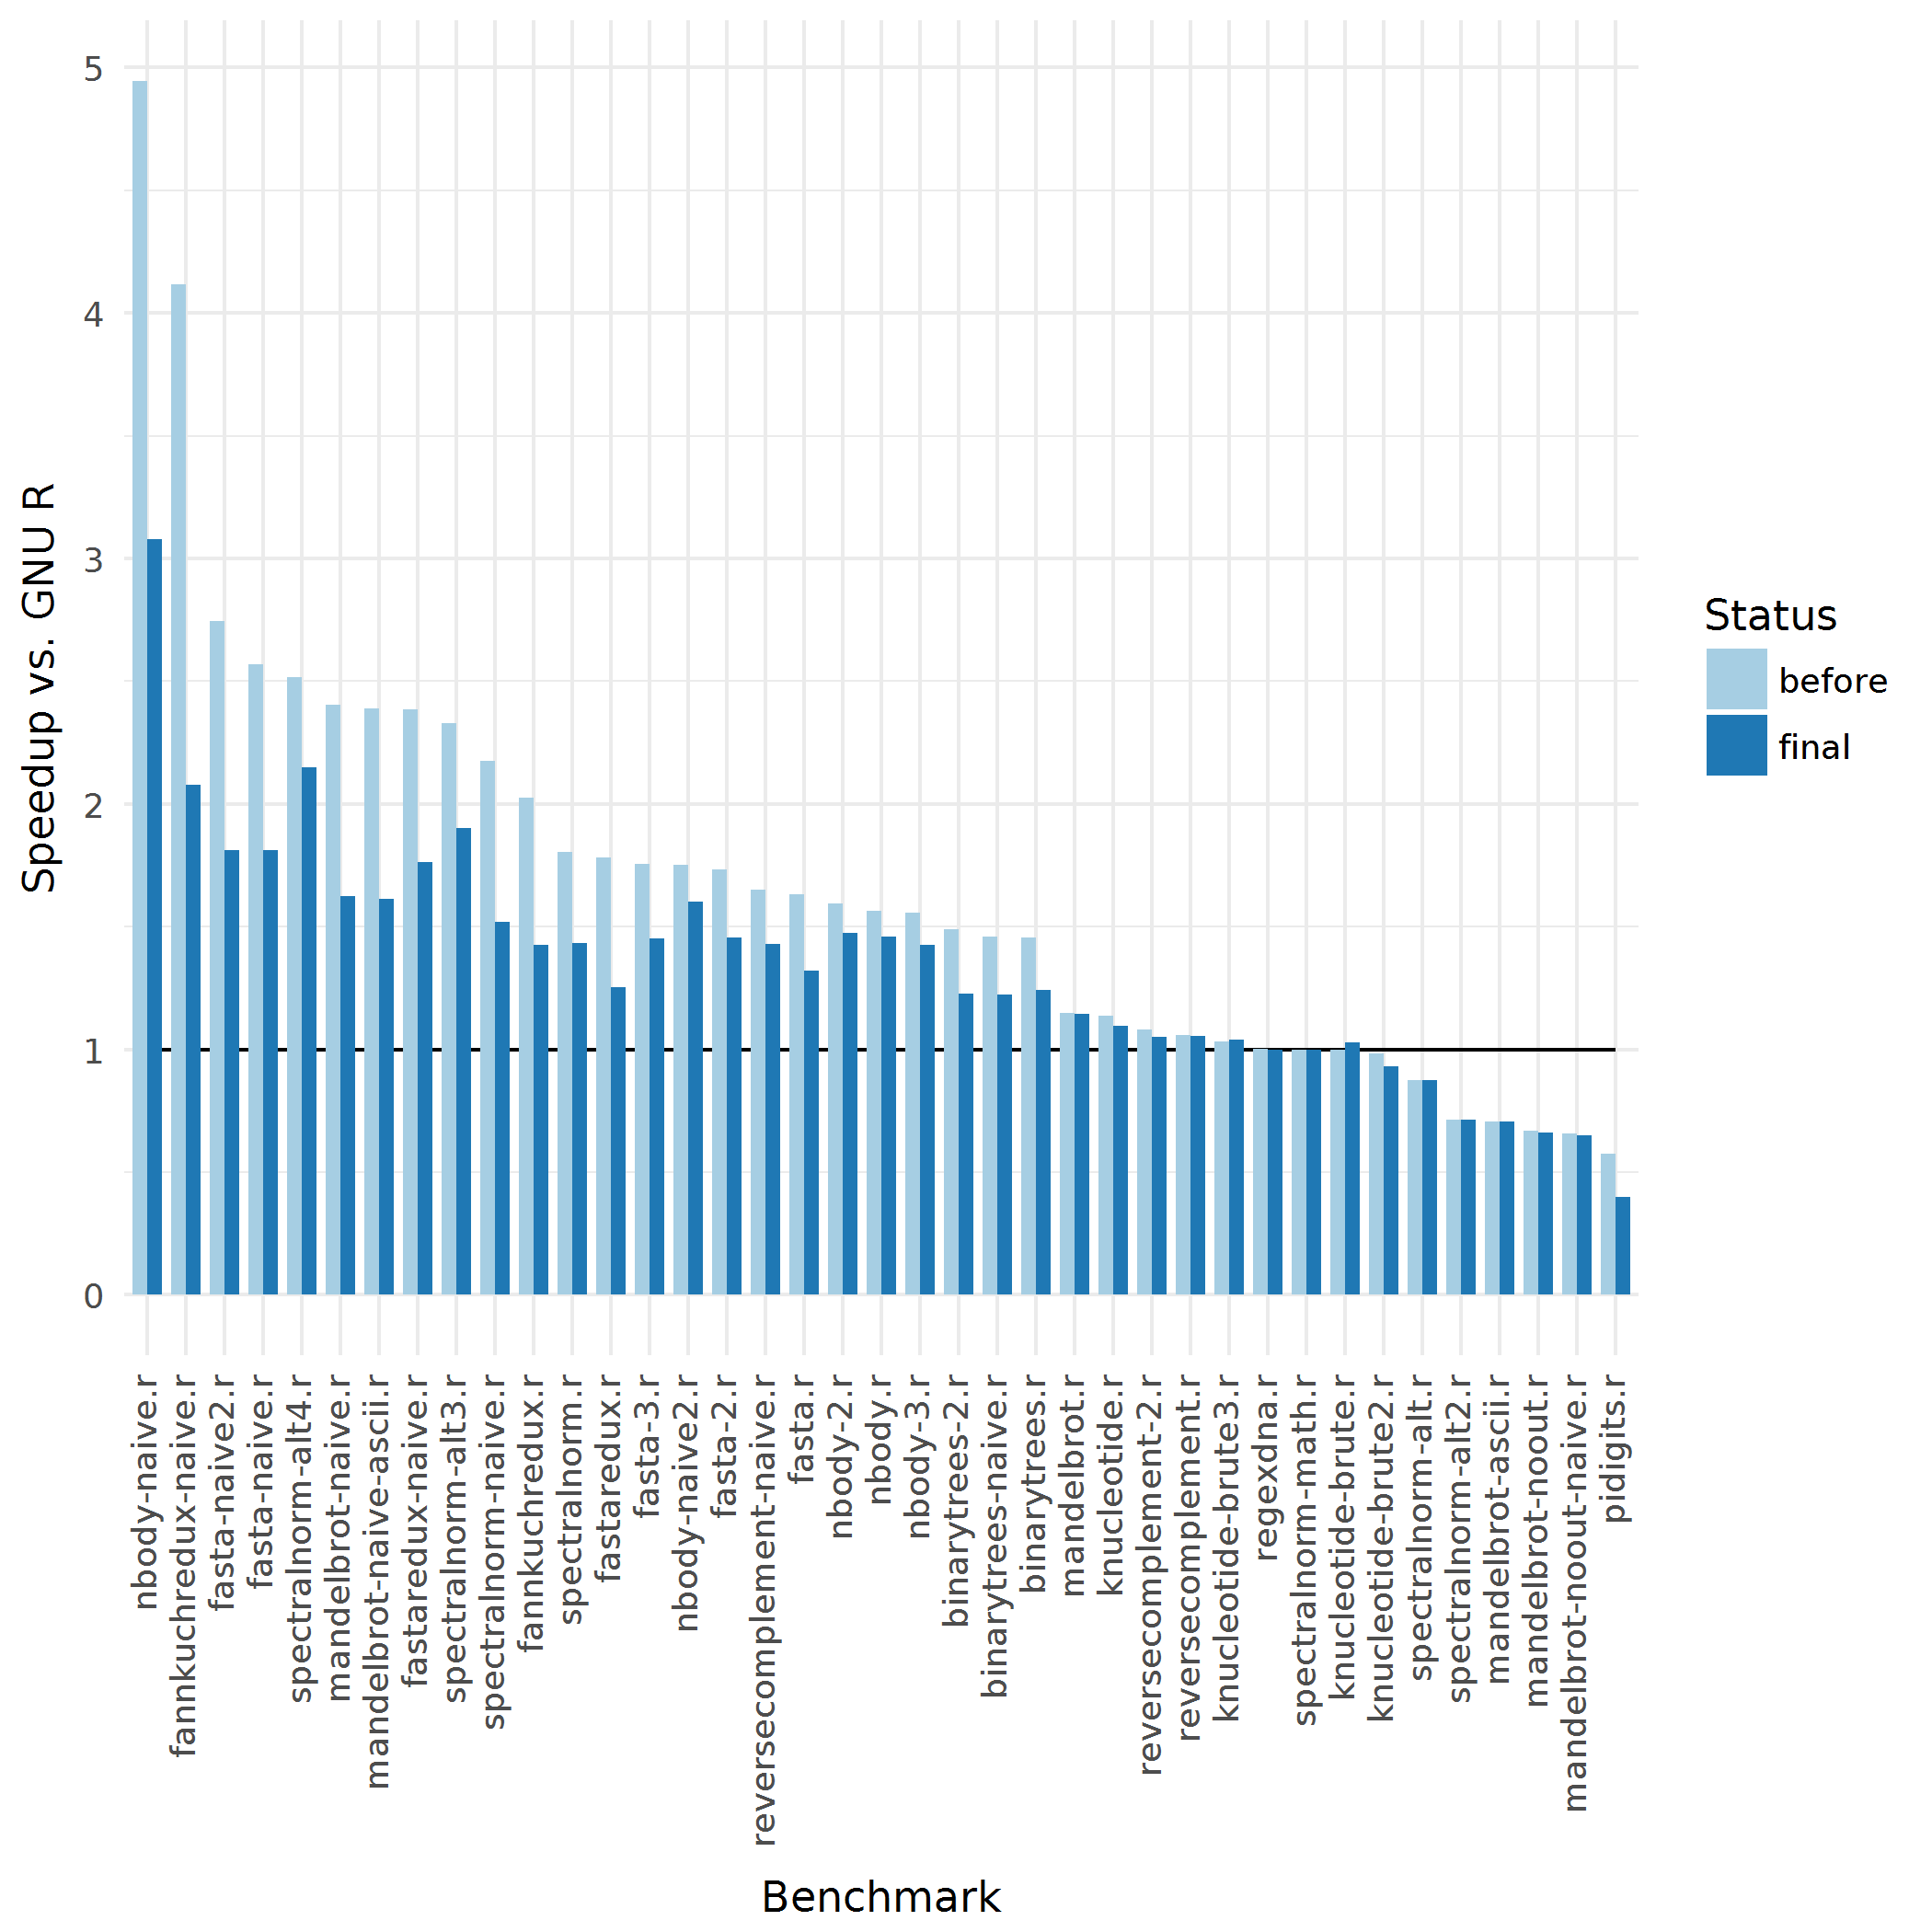
\includegraphics[width=\linewidth]{images/overall}}
\end{figure}

The lighter color refers to the state before anything was done, the darker after all the changes described in chapter \ref{improvements}.

The slowdowns are computed relative to the running time of GNU R byte-compiled code, which was normalized to 1 (this is indicated by the solid black line).

It can be clearly seen that the most speedup was gained in the naive implementations.

Overall, an average slowdown of about 1.678 against GNU R was lowered to about 1.336.

Figure \ref{fig:history} captures the running times of each benchmark over the course of the work described in chapter \ref{improvements}.

\begin{figure}[htbp]
  \caption{\label{fig:history}History of running times}
  \centering
  \tmpframe{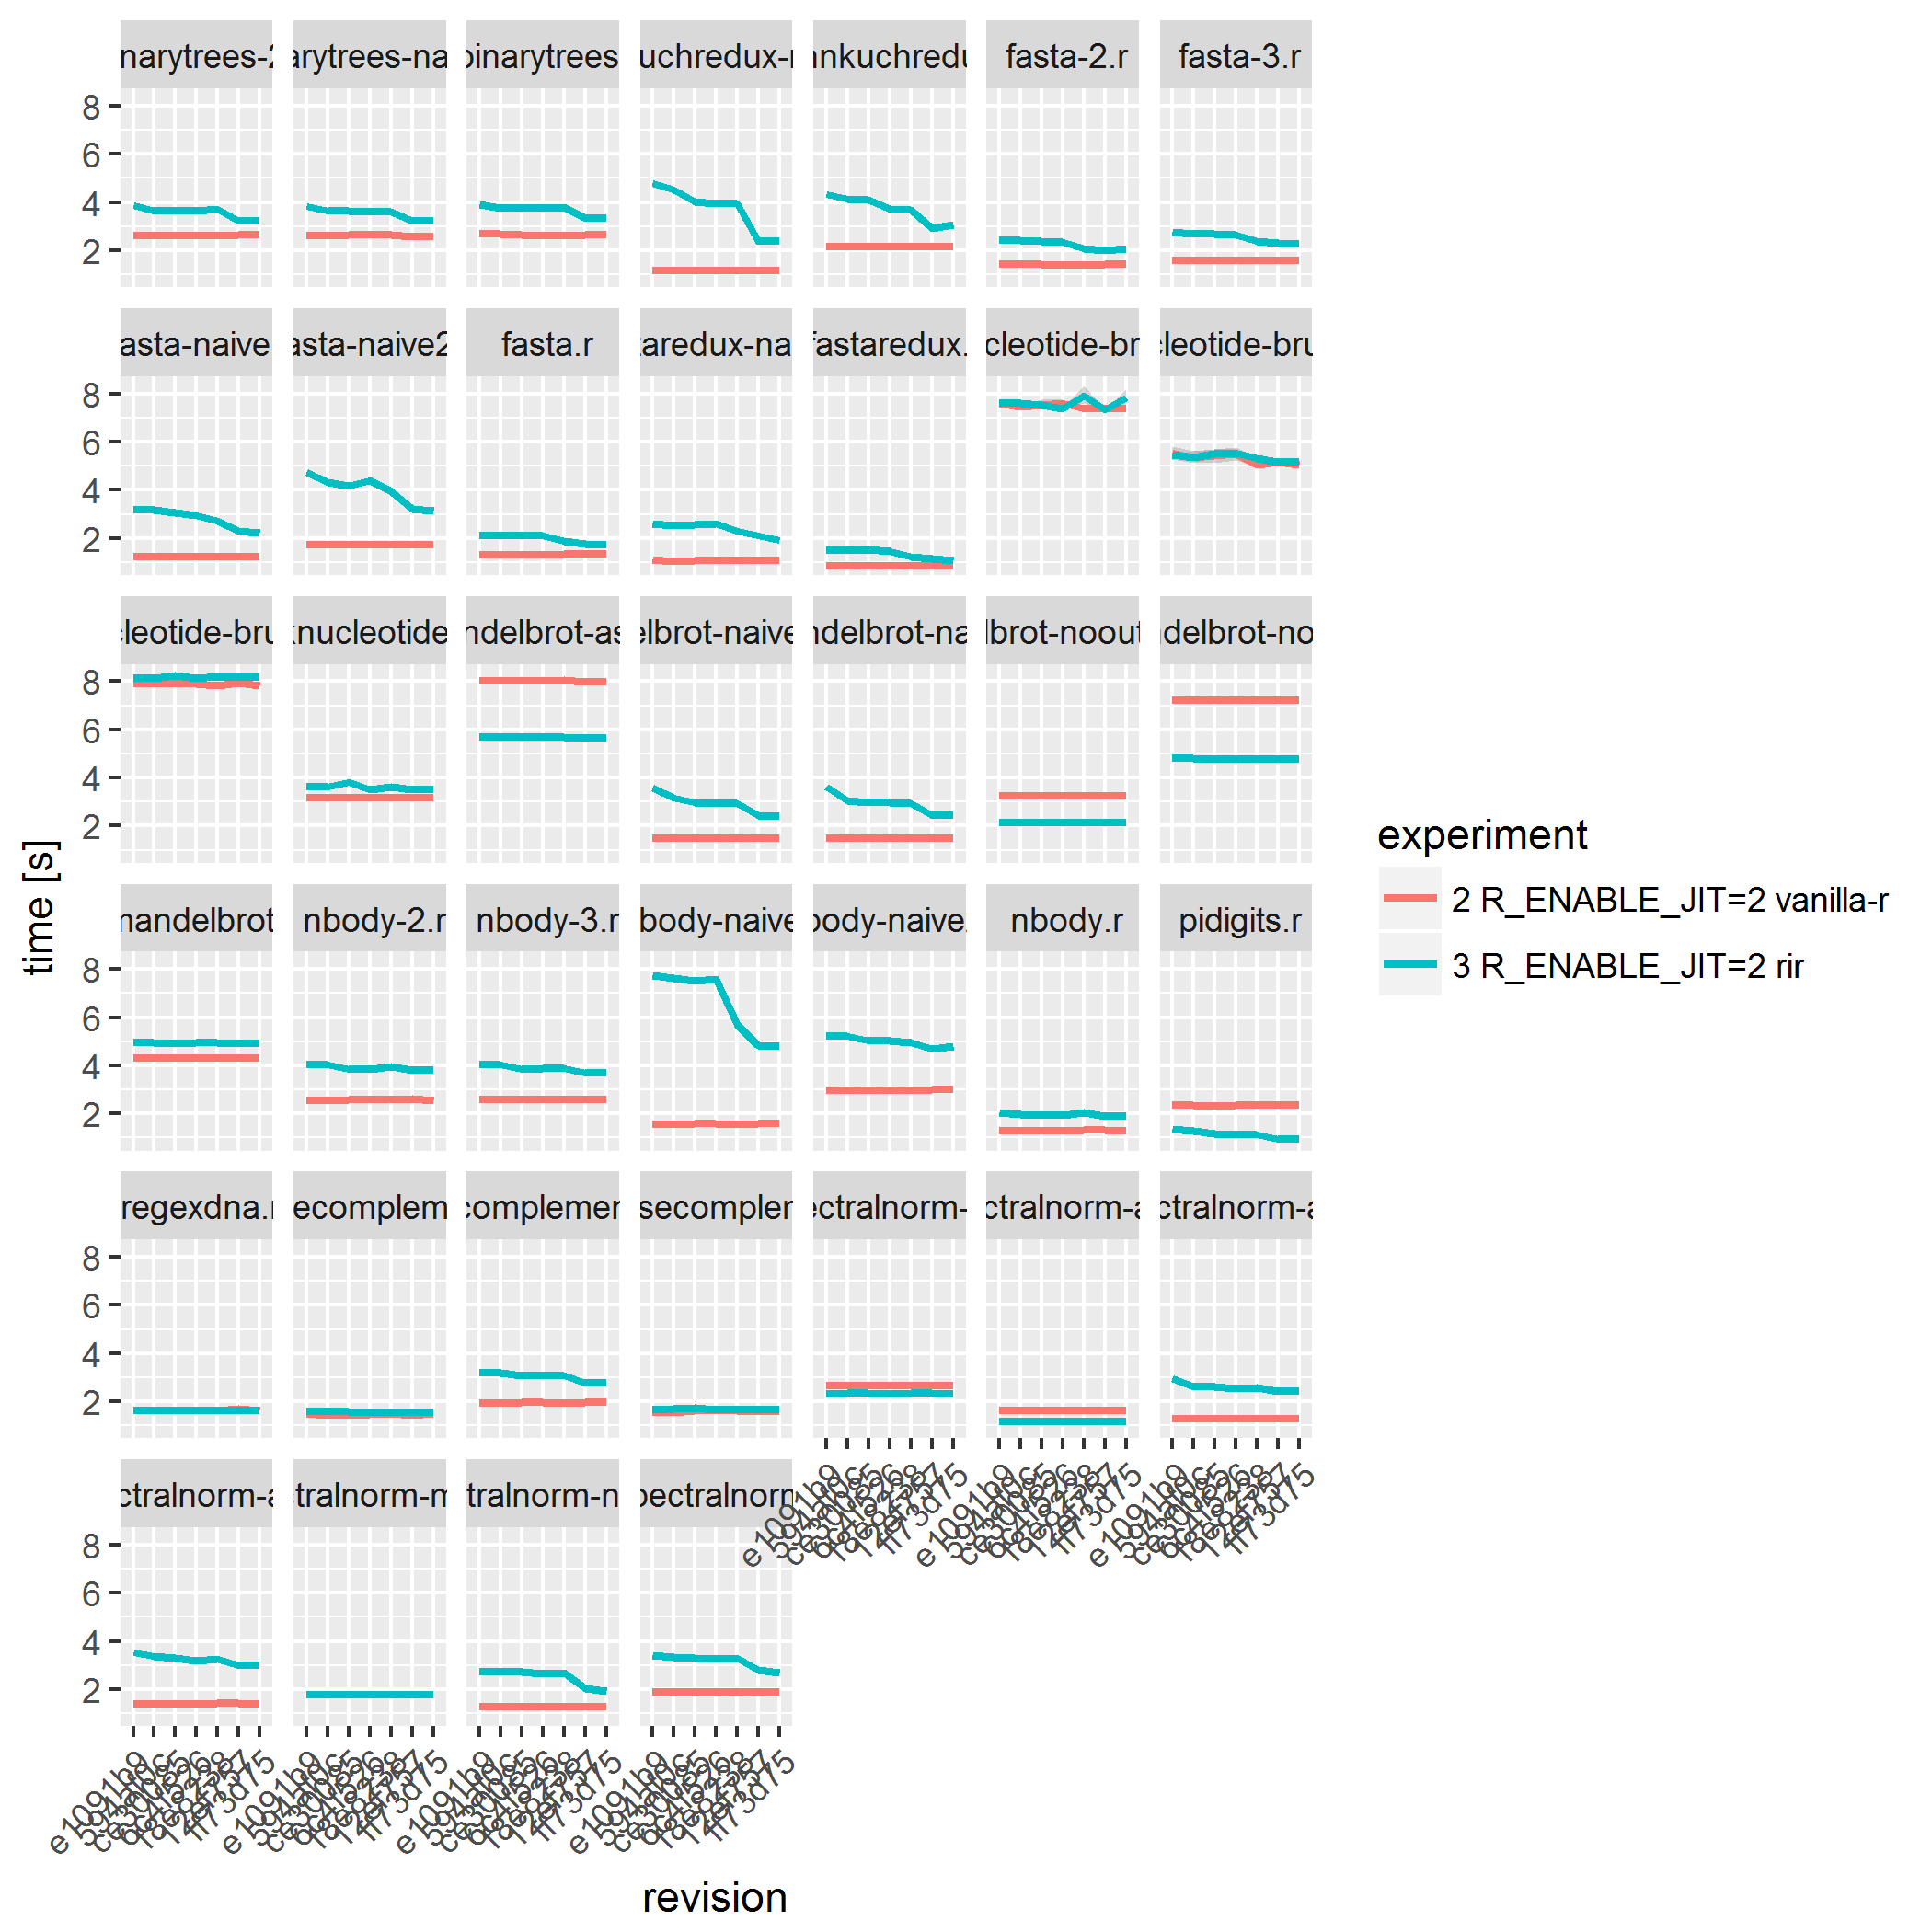
\includegraphics[width=\linewidth]{images/speedup_history}}
\end{figure}

In the figure, the light blue color represents the performance of the GNU R bytecode. As all measurments were carried out on the same version of GNU R (namely 3.3.2) the times are identical.

For three mandelbrot, pidigits and two spectralnorm benchmarks RIR was already faster.

Knucleotide fastanaive some slowdowns.

Some mandelbrot, regexdna, spectralnorm, reversecomplement have not changed at all.

Nbody naive \todo[add plot] big drop interpreter refactoring. also fasta naive, fannkuchrecux naive, spectralnorm naive and others. describe what kind of code they are

\begin{figure}[htbp]
  \caption{\label{fig:}\todo}
  \centering
  \tmpframe{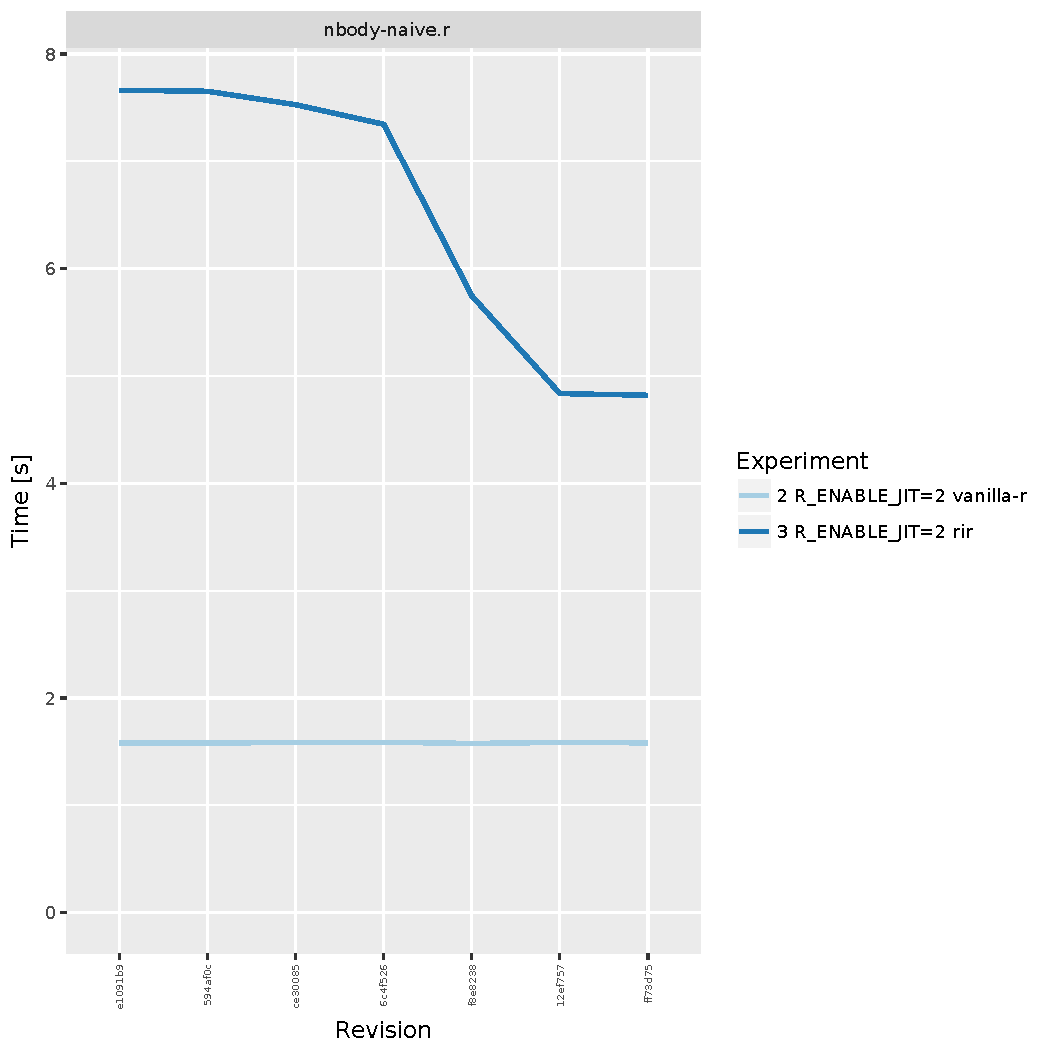
\includegraphics[width=\linewidth]{images/nbody-naive}}
\end{figure}

\begin{figure}[htbp]
  \caption{\label{fig:}\todo}
  \centering
  \tmpframe{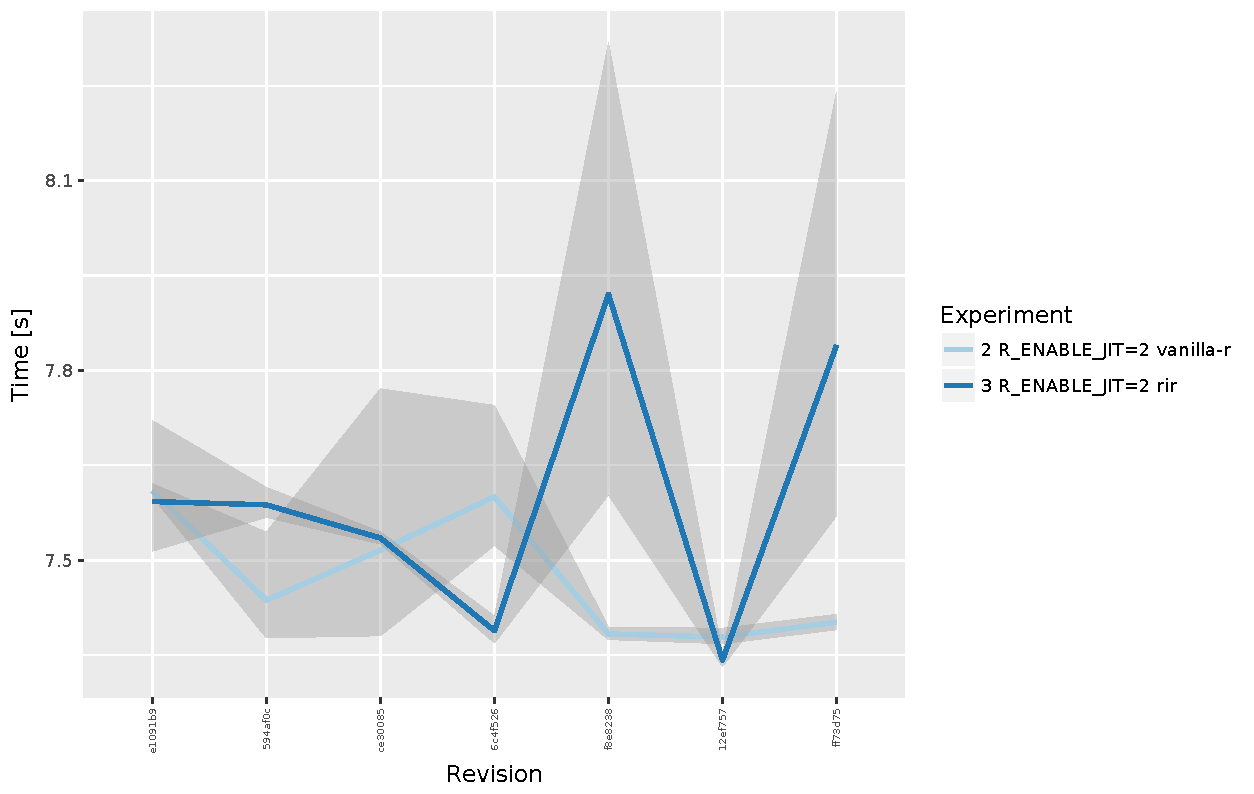
\includegraphics[width=\linewidth]{images/knucleotide-brute}}
\end{figure}

\begin{figure}[htbp]
  \caption{\label{fig:}\todo}
  \centering
  \tmpframe{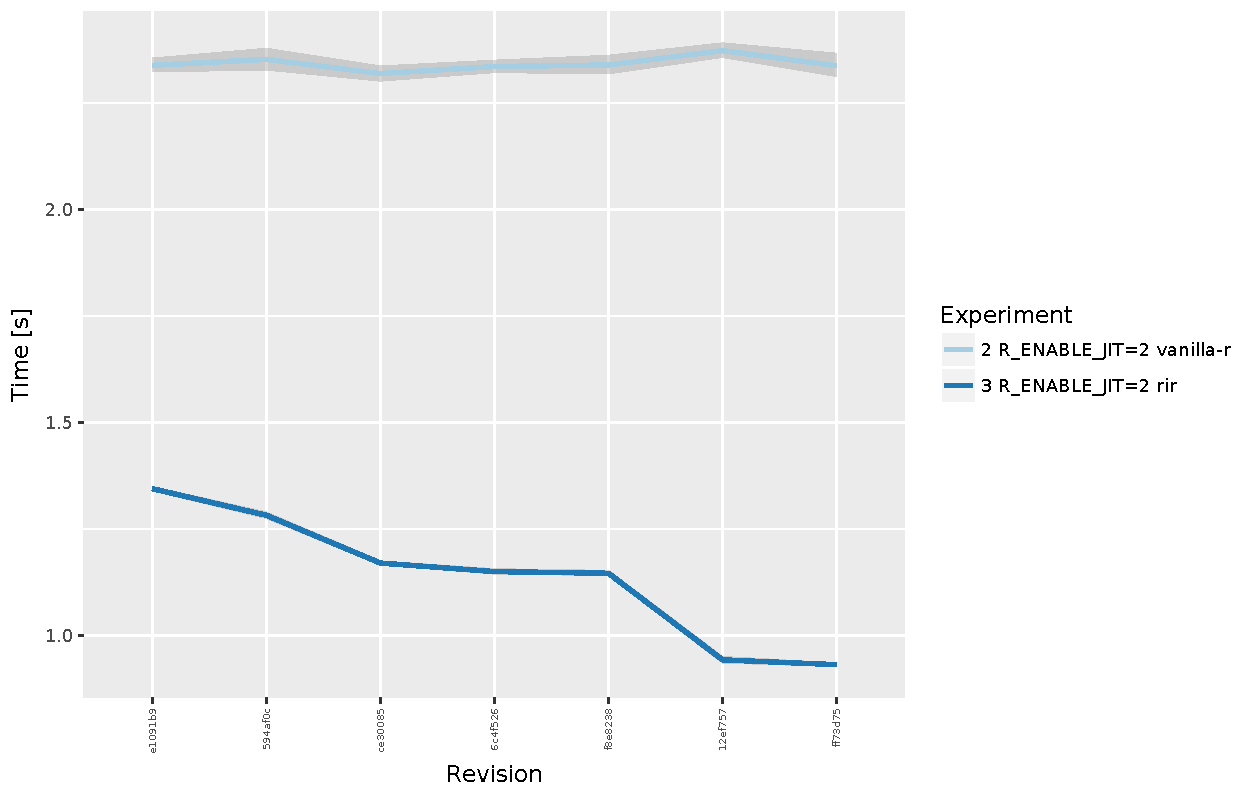
\includegraphics[width=\linewidth]{images/pidigits}}
\end{figure}

Why pidigits so fast and why it improved further

The average speedup versus GNU R over the measured revisions is captured in figure \ref{fig:avg-speedup-history}.

\begin{figure}[htbp]
  \caption{\label{fig:avg-speedup-history}History of average speedup vs. GNU R}
  \centering
  \tmpframe{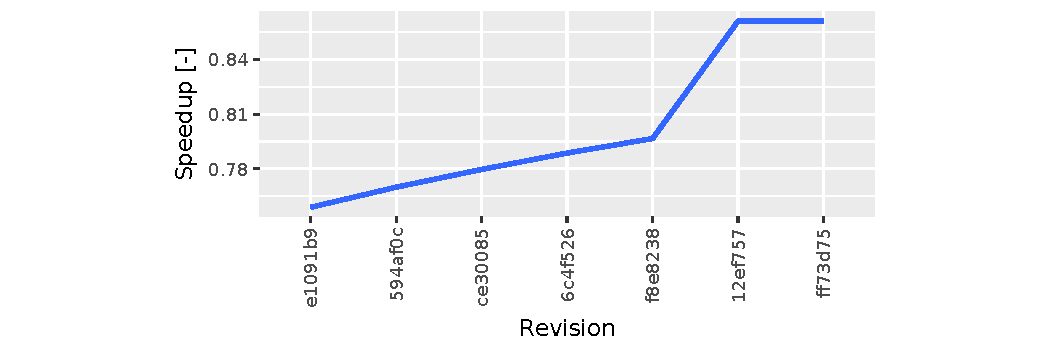
\includegraphics[width=\linewidth]{images/avg_speedup}}
\end{figure}

Additionaly, for ensuring that the improvements had positive effects, usually a kind of microbenchmark, such as the one in listing \ref{lst:microbench}, were checked by hand in fresh sessions of GNU R (with JIT disabled and with JIT set to 2) and RIR (with JIT enabled). In the code, a function is defined and measured repeatedly. The final reported time is computed as arithmetic mean of only a tailing part of the runs. This is to ensure a proper warmup (i.e. everything is byte-compiled by the JIT and possibly the processor branch predictors warm up).

\begin{listing}[htbp]
  \caption{\label{lst:microbench}Microbenchmark code}
  \begin{rcode}
f <- function() {
    i <- 10000000L
    while (i > 0) i <- i - 1
}
t <- c()
for (x in 1:10) t <- c(t, system.time(f())[[3]])
mean(t[5:10])
  \end{rcode}
\end{listing}

In this way, it was for instance found that threaded code starts to pay off only for larger programs.


\begin{conclusion}
\label{conclusion}
\todo[conclusion, future work, related work, fails - stoke etc.]

\end{conclusion}

\printbibliography

\appendix

\chapter{Acronyms}
\printglossary[type=\acronymtype,style=acronyms]

\chapter{Contents of the enclosed CD}

\vfill

\todo[contents of cd]
\blind[1]

%\begin{dirfigure}%
%    \dirtree{%
%        .1 README.md\DTcomment{stručný popis obsahu média}.
%        .1 src.
%            .2 utvsapi-benchmark\DTcomment{skripty pro měření rychlosti}.
%                .3 logs\DTcomment{záznamy z~měření rychlosti}.
%            .2 utvsapi-django\DTcomment{implementace ukázkové služby v~DRF}.
%            .2 utvsapi-eve\DTcomment{implementace ukázkové služby v~Eve}.
%            .2 utvsapi-ripozo\DTcomment{implementace ukázkové služby v~ripozu}.
%            .2 utvsapi-sandman\DTcomment{implementace ukázkové služby v~sandmanu2}.
%            .2 utvsapitoken\DTcomment{společný modul pro práci s~tokenem}.
%            .2 diplomka\DTcomment{zdrojová forma práce ve formátu Markdown a \XeLaTeX{}}.
%        .1 DP\_Hroncok\_Miroslav\_2016.pdf\DTcomment{text práce ve formátu PDF}.
%    }
%\caption{Obsah přiloženého média}
%\end{dirfigure}


\end{document}
